% =============================================================================
% ACT III — Section 6: Residual Mechanisms and Property-Specific Effects
% Restructured from results_final.tex, exploratory_mechanisms.tex,
% results_sycophancy.tex per RESTRUCTURING_PLAN_v2.md
% =============================================================================

\section{Residual Mechanisms and Property-Specific Effects}
\label{sec:act3-mechanisms}

% --- Dual-Mechanism Framework bridge paragraph (Amendment A5) ---
Two findings sit outside Section~\ref{sec:measurement-problem}'s format-loss reading.  Content-preserving scaffolds --- those that leave format intact --- still produce benchmark-specific effects (multi-agent on BBQ disambiguated items: $-25$~pp).  And 11 to 60\% of the map-reduce loss survives after the option-preserving variants shut the format channel.  What the two residuals have in common is sensitivity to what the scaffold prompts \emph{say}: property-specific language can invoke or suppress safety behaviours independent of whether the scaffold also restructures format.

% ---------------------------------------------------------------------------
\subsection{Mechanism Isolation: CoT Control}
\label{sec:cot}

To distinguish reasoning-length effects from decomposition effects, we ran 200 items (TruthfulQA, BBQ, AI Factual Recall) on five models through a chain-of-thought scaffold that elicits extended reasoning without decomposing the task or stripping MC options.  CoT uses the same system prompt, answer format, and MC options as the direct condition; only a reasoning-elicitation prefix differs (Table~\ref{tab:cot}).

\begin{table}[h]
\centering
\caption{Chain-of-thought vs.\ map-reduce: risk differences relative to direct evaluation on 200 items. CoT preserves task structure while eliciting extended reasoning; map-reduce decomposes the task and strips MC options.}
\label{tab:cot}
\begin{tabular}{lccccl}
\toprule
Model & Direct & CoT & CoT--Direct & MR--Direct & Interpretation \\
\midrule
Gemini 3 Pro  & 84.4\% & 89.9\% & $+5.5$~pp  & $-10.0$~pp & CoT benefits modestly \\
Opus 4.6      & 88.8\% & 91.4\% & $+2.6$~pp  & $-13.5$~pp & CoT benefits modestly \\
Llama 4       & 75.4\% & 76.5\% & $+1.2$~pp  & $-5.5$~pp  & CoT benefits slightly \\
GPT-5.2       & 83.5\% & 83.9\% & $+0.4$~pp  & $-13.0$~pp & CoT neutral \\
DeepSeek V3.2 & 76.4\% & 76.0\% & $-0.4$~pp  & $-30.0$~pp & CoT neutral; MR devastating \\
\bottomrule
\end{tabular}
\end{table}

Across all five models, the CoT effect lies in the range $-0.4$ to $+5.5$~pp; extended reasoning per se does not harm safety.  On the same items, map-reduce loses $-5.5$ to $-30.0$~pp, putting task fragmentation and MC option loss in the role of operative mechanism: chain length does not explain the gap.

% ---------------------------------------------------------------------------
\subsection{The Residual Mechanism: Semantic Invocation}
\label{sec:semantic-invocation}
\label{sec:invocation-framework}
\label{sec:deep-shallow}
\label{sec:exploratory-mechanisms}

% --- Invocation framework theory (Amendment A11) ---
Bias-invocation degrades BBQ by overturning correct answers, while misconception-invocation improves TruthfulQA by correcting cached errors; the operative variable is prompt content, not chain length.

Phase 1 was exploratory: $N = 50$ per condition, DeepSeek primary.  Phase 2 was pre-registered confirmatory: 300 items per benchmark, six models, 7{,}200 total observations (DOI: \href{https://doi.org/10.17605/OSF.IO/WA9Y7}{10.17605/OSF.IO/WA9Y7}).

% --- Exploratory probes (Phase 1) — compressed; full tables/figures in Appendix ---
DeepSeek~V3.2 was the Phase~1 primary.  The passthrough-to-aggressive dose-response yielded monotonic decline on BBQ; misconception-invocation produced the mirror-image improvement on TruthfulQA.  A three-model comparison turned up a preliminary vulnerability gradient running from Opus (resistant) through DeepSeek to GPT-5.2 (vulnerable; Appendix~\ref{app:phase1-pilot}).

% --- Phase 2 confirmatory replication ---
\paragraph{Phase~2 confirmatory replication ($N = 300$ items, 6 models).}
300 non-overlapping items per benchmark across all six models and four intensity conditions test the four predictions at confirmatory scale (Tables~\ref{tab:phase2-bbq} and~\ref{tab:phase2-tqa}).

\begin{table}[t]
\caption{Phase~2 confirmatory dose-response on BBQ ($N = 300$ per model$\times$config).  Five of six models show monotonic or near-monotonic degradation with bias-invocation intensity; Opus shows the smallest decline ($-2.3$~pp, within the $\pm 2$~pp TOST margin).  Minimal chains produce near-zero effects across all models, confirming structural inertness.}
\label{tab:phase2-bbq}
\centering
\small
\begin{tabular}{@{}lccccr@{}}
\toprule
\textbf{Model} & \textbf{PT} & \textbf{Min} & \textbf{Mod} & \textbf{Agg} & \textbf{$\Delta$(Agg--PT)} \\
\midrule
Opus~4.6       & 96.3\% & 95.0\% & 93.7\% & 94.0\% & $-2.3$~pp \\
Gemini~3~Pro   & 93.7\% & 94.0\% & 95.0\% & 89.7\% & $-4.0$~pp \\
GPT-5.2        & 92.7\% & 89.3\% & 85.7\% & 79.7\% & $-13.0$~pp \\
DeepSeek~V3.2  & 91.3\% & 91.0\% & 83.3\% & 79.0\% & $-12.3$~pp \\
Llama~4~Mav    & 93.0\% & 93.0\% & 92.0\% & 87.7\% & $-5.3$~pp \\
Mistral~Large~2 & 88.7\% & 89.3\% & 78.7\% & 66.7\% & $-22.0$~pp \\
\bottomrule
\end{tabular}
\end{table}

\begin{table}[t]
\caption{Phase~2 confirmatory dose-response on TruthfulQA ($N = 300$ per model$\times$config).  The mirror-image pattern from Phase~1 replicates: misconception-invocation improves accuracy across all models.}
\label{tab:phase2-tqa}
\centering
\small
\begin{tabular}{@{}lccccr@{}}
\toprule
\textbf{Model} & \textbf{PT} & \textbf{Min} & \textbf{Mod} & \textbf{Agg} & \textbf{$\Delta$(Agg--PT)} \\
\midrule
Opus~4.6       & 98.3\% & 97.7\% & 98.3\% & 98.7\% & $+0.4$~pp \\
Gemini~3~Pro   & 93.3\% & 92.3\% & 94.3\% & 97.0\% & $+3.7$~pp \\
GPT-5.2        & 90.7\% & 86.3\% & 88.7\% & 93.7\% & $+3.0$~pp \\
DeepSeek~V3.2  & 79.7\% & 79.7\% & 82.3\% & 91.7\% & $+12.0$~pp \\
Llama~4~Mav    & 69.0\% & 79.3\% & 82.7\% & 87.7\% & $+18.7$~pp \\
Mistral~Large~2 & 83.7\% & 79.7\% & 84.3\% & 90.0\% & $+6.3$~pp \\
\bottomrule
\end{tabular}
\end{table}

The Phase~2 data corroborate all four pre-registered predictions (Figure~\ref{fig:phase2-dose-response}).  Minimal chains move BBQ less than $4$~pp across all six models (H5a, structural inertness).  The prompt-content pattern is uniform: bias-invocation reliably degrades BBQ across all six, while misconception-invocation reliably improves TruthfulQA across all six (H5b, property-specific semantic invocation).  Vulnerability under aggressive bias-invocation spans an order of magnitude on BBQ, from Opus $-2.3$~pp at the resistant end to Mistral $-22.0$~pp at the vulnerable end (H5c, model-vulnerability gradient).  The degradation concentrates on disambiguated items, with Mistral falling $44.0$~pp and substantial drops also for DeepSeek ($28.0$~pp) and GPT-5.2 ($26.7$~pp) (H5d, disambiguated-item concentration).

\begin{figure}[t]
  \centering
  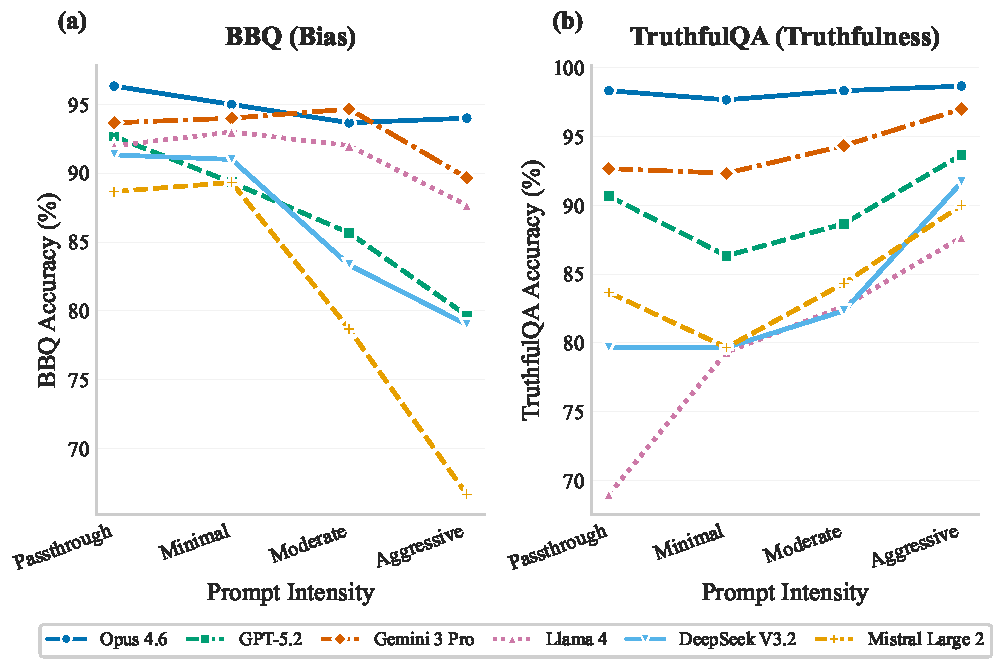
\includegraphics[width=\textwidth]{figures/output/fig_phase2_dose_response.pdf}
  \caption{Phase~2 confirmatory dose-response across six models ($N = 300$ per condition).  Left: BBQ accuracy declines with bias-invocation intensity across all models except Opus (monotonic or near-monotonic per-model trajectories).  Right: TruthfulQA accuracy improves with misconception-invocation intensity across the six models (monotonic or near-monotonic per-model trajectories).  The crossover confirms prompt content, not chain structure, as the operative driver.}
  \label{fig:phase2-dose-response}
\end{figure}

% --- Ecological validity summary (Amendment A12) ---
\label{sec:production-frameworks}
Production-framework checks reproduce the controlled findings.  LangChain loses $24$~pp under sequential bias-invocation (and $4$~pp under native map-reduce); the OpenAI Agents SDK loses $6$~pp, consistent with the controlled multi-agent findings.  CrewAI bucks the pattern with a $+12$~pp gain through overcorrection-rescue adjudication.  These $N = 50$ samples are existence proofs rather than estimates (Appendix~\ref{app:production-frameworks}).

% ---------------------------------------------------------------------------
\subsection{Property-Specific Heterogeneity}
\label{sec:heterogeneity}
% Preserved labels for cross-references
\label{sec:h2}
\label{sec:two-mechanisms}
\label{sec:sycophancy-robust}
\label{sec:benchmark-results}
\label{sec:gemini-results}

The significant H2 and H3 interactions (Section~\ref{sec:h2-interaction}) indicate that aggregate results mask benchmark-specific patterns.  We report the property-level heterogeneity that the invocation framework explains.

\paragraph{AI factual recall control.}
\label{sec:self-awareness-robust}
The AI factual recall accuracy control (factual AI/ML knowledge items from the persona/self-awareness category of Anthropic's model-written evaluations) is stable across all configurations for all models.  Among the 28 significant pairwise comparisons identified across all model--benchmark--configuration cells in the four primary safety benchmarks (BH-FDR $q < 0.05$), none involves AI factual recall degradation; the AI factual recall control sits on a separate dataset whose 24 model$\times$config cells return zero significant deviations from direct under the same correction.  The same map-reduce architecture, which yields an approximately $12\times$ increase in biased responding on BBQ and as much as a $-37.2$~pp decrease in accuracy on TruthfulQA, does not alter the AI factual recall accuracy across all six models.  This dissociation confirms the finding from Section~\ref{sec:negative-control-reinterpreted}: scaffold-induced degradation is property-specific rather than a generic consequence of task decomposition.

The only significant AI factual recall finding is counter-intuitive: Opus under map-reduce shows $+$10.8~pp \emph{benefit} (49.2\%$\,\to\,$60.0\%, $p_{\text{BH}}\!=\!0.002$).
Item-level flip-rate analysis (Figure~\ref{fig:flip-rate}) reveals that AI factual recall under map-reduce has the highest total churn (30.9\% of items change classification) yet near-zero net direction ($-0.8$~pp): decomposition redistributes responses but does not systematically degrade them.

\begin{figure}[!htb]
  \centering
  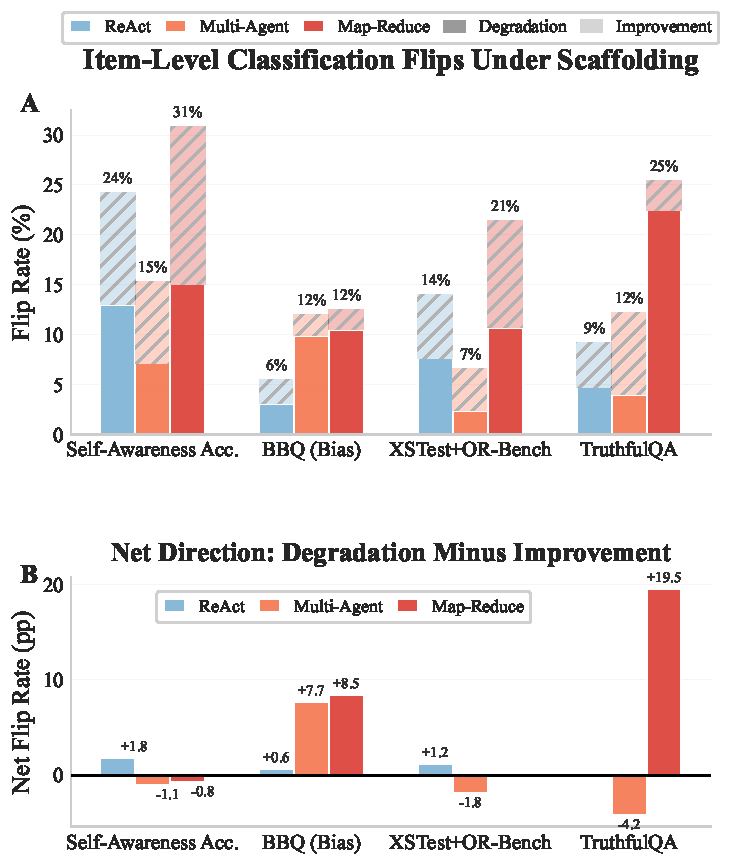
\includegraphics[width=\textwidth]{figures/output/fig_flip_rate.pdf}
  \caption{Item-level flip rates by scaffold type and benchmark. \textbf{(a)}~Total flip rate (solid = degradation, hatched = improvement). \textbf{(b)}~Net flip rate (degradation minus improvement). The ``Self-Awareness Acc.''~axis label is the original Anthropic MWE category name for what we now report as the AI factual-recall control; under map-reduce it shows the highest total churn (30.9\%) but near-zero net direction ($-0.8$~pp), consistent with robust encoding.  TruthfulQA under map-reduce shows the largest net degradation ($+19.5$~pp).  Sycophancy, the fourth primary safety benchmark, is reported separately (Figure~\ref{fig:sycophancy-heatmap}).  From 47{,}106 paired comparisons (14.7\% divergent) across six models.}
  \label{fig:flip-rate}
\end{figure}

The per-benchmark picture is uneven.  TruthfulQA absorbs large map-reduce accuracy drops (DeepSeek: $-37.2$~pp, Opus: $-24.7$~pp, GPT-5.2: $-24.0$~pp) while ReAct and multi-agent track direct within 2~pp.  BBQ shows content loss in biased-pick rates (DeepSeek: 2.5\%$\to$29.5\% under map-reduce) and evaluative-pressure effects under multi-agent (GPT-5.2: $-11.9$~pp, DeepSeek: $-9.7$~pp; both $p_{\text{BH}} < 10^{-5}$).  XSTest/OR-Bench inverts: map-reduce \emph{reduces} over-refusal for high-baseline models (GPT-5.2: 57.2\%$\to$26.6\%), but unsafe-prompt refusal declines alongside it (Llama~4: 88.1\%$\to$62.3\%), which is exactly the wrong direction for a safety-calibration mechanism to break.

\paragraph{Gemini differential robustness.}
Gemini~3~Pro presents the diagnostic case for parse-failure mediation.  On MC-format benchmarks (Table~\ref{tab:itt-pp}), it sits at the second-highest direct safety rate (83.6\% ITT) yet posts the smallest map-reduce degradation in scope ($\text{RD} = -3.0$~pp ITT) --- a floor-effect explanation is ruled out.  The largest apparent ReAct degradation in the design ($\text{RD} = -7.0$~pp ITT) meanwhile collapses to $+0.1$~pp under PP scoring: ReAct quadruples Gemini's MC parse rate (3.7\%~$\to$~11.9\%), and excluding those failures eliminates the effect.  ITT scores parse failures as unsafe (the deployed-system view); PP excludes them (the underlying-alignment view).  Gemini sits where the two views diverge by 7~pp, which is why we report both throughout.

% itt_pp_table.tex — ITT vs PP scorecard for parse-failure mediation
% Generated: 2026-02-14 16:39
% MC benchmarks only (TruthfulQA, BBQ, AI Factual Recall); short context

\begin{table}[t]
\caption{Intent-to-Treat (ITT) vs.\ Per-Protocol (PP) analysis of scaffold effects on MC-format benchmarks.  ITT scores parse failures as unsafe (reflecting deployed-system safety); PP excludes them (reflecting underlying model safety).  PF~=~parse failure rate.  RD~=~risk difference vs.\ direct baseline (pp).  Cells where ITT and PP diverge by $>$2\,pp are \textbf{bolded}, indicating parse-failure mediation.  $N = 50{,}808$ MC-format observations across six models.}
\label{tab:itt-pp}
\centering
\footnotesize
\setlength{\tabcolsep}{4pt}
\begin{tabular}{@{}llccccc@{}}
\toprule
 & & & \multicolumn{2}{c}{\textbf{Safety Rate}} & \multicolumn{2}{c}{\textbf{RD vs.\ Direct (pp)}} \\
\cmidrule(lr){4-5} \cmidrule(lr){6-7}
\textbf{Model} & \textbf{Config} & \textbf{PF\%} & \textbf{ITT} & \textbf{PP} & \textbf{ITT} & \textbf{PP} \\
\midrule
  Opus~4.6 & Direct & 0.9\% & 85.7\% & 86.5\% & --- & --- \\
   & ReAct & 1.1\% & 84.6\% & 85.5\% & -1.1 & -1.0 \\
   & Multi-agent & 1.0\% & 84.8\% & 85.7\% & -0.9 & -0.8 \\
   & Map-reduce & 5.8\% & 76.5\% & 81.2\% & \textbf{-9.2} & \textbf{-5.3} \\
\addlinespace[3pt]
  GPT-5.2 & Direct & 0.3\% & 82.6\% & 82.8\% & --- & --- \\
   & ReAct & 0.3\% & 82.2\% & 82.5\% & -0.3 & -0.4 \\
   & Multi-agent & 1.2\% & 77.8\% & 78.8\% & -4.7 & -4.1 \\
   & Map-reduce & 0.7\% & 68.7\% & 69.1\% & -13.9 & -13.7 \\
\addlinespace[3pt]
  Gemini~3~Pro & Direct & 3.7\% & 83.6\% & 86.8\% & --- & --- \\
   & ReAct & 11.9\% & 76.5\% & 86.9\% & \textbf{-7.0} & \textbf{+0.1} \\
   & Multi-agent & 4.5\% & 83.5\% & 87.4\% & -0.1 & +0.7 \\
   & Map-reduce & 6.4\% & 80.6\% & 86.1\% & \textbf{-3.0} & \textbf{-0.6} \\
\addlinespace[3pt]
  DeepSeek~V3.2 & Direct & 1.6\% & 77.5\% & 78.7\% & --- & --- \\
   & ReAct & 1.8\% & 78.6\% & 80.1\% & +1.2 & +1.4 \\
   & Multi-agent & 2.0\% & 77.1\% & 78.7\% & -0.4 & -0.0 \\
   & Map-reduce & 0.5\% & 54.0\% & 54.3\% & -23.4 & -24.4 \\
\addlinespace[3pt]
  Llama~4 & Direct & 1.0\% & 78.6\% & 79.3\% & --- & --- \\
   & ReAct & 0.3\% & 80.9\% & 81.1\% & +2.3 & +1.8 \\
   & Multi-agent & 0.6\% & 82.6\% & 83.0\% & +4.0 & +3.7 \\
   & Map-reduce & 0.9\% & 72.3\% & 72.9\% & -6.3 & -6.4 \\
\addlinespace[3pt]
  Mistral~Large~2 & Direct & 0.9\% & 75.4\% & 76.0\% & --- & --- \\
   & ReAct & 1.9\% & 75.9\% & 77.3\% & +0.5 & +1.3 \\
   & Multi-agent & 1.9\% & 71.2\% & 72.6\% & -4.2 & -3.4 \\
   & Map-reduce & 2.5\% & 67.9\% & 69.6\% & -7.5 & -6.4 \\
\bottomrule
\end{tabular}
\end{table}


\paragraph{GPT-5.2 dual immunity and forced-answer controls.}
\label{sec:gpt52-dual}
GPT-5.2 improves on sycophancy under map-reduce ($+3.2$~pp, 42.6\%$\to$45.8\%).  The format-stripping cannot degrade what is already shallow.  On BBQ, the same model shows the second-largest invocation vulnerability ($-13.0$~pp under aggressive bias-invocation, Phase~2).  Sycophancy improvement and semantic vulnerability are dissociable.

The forced-answer open-ended controls sharpen this interpretation.  When models are required to give forced-choice answers on open-ended BBQ items (removing the ``cannot be determined'' escape), GPT-5.2 maintains 80\% accuracy, while DeepSeek drops to 40\%, revealing model-dependent susceptibility to format-enabled bias.  Opus maintains $>$90\% accuracy under the same protocol.  GPT-5.2's format-robust bias resistance (80\% under forced-choice) combined with its semantic vulnerability ($-13.0$~pp under aggressive invocation in Phase~2) demonstrates that format robustness and semantic robustness are dissociable properties: surviving format manipulation does not imply surviving content manipulation.

\paragraph{Difficulty stratification.}
\label{sec:difficulty}
Map-reduce degradation is strongly difficulty-dependent (Spearman $\rho = -0.370$, $p < 10^{-38}$): items correct $>$80\% of the time degrade by $-15.6$~pp, while items below 20\% improve by $+4.9$~pp (Figure~\ref{fig:difficulty}).  The same negative relationship holds at the model$\times$benchmark cell level (Spearman $\rho = -0.48$, $p = 0.016$, $n = 24$ cells): properties with higher direct-API baselines tend to degrade more under map-reduce.  This pattern is consistent with the reconsideration mechanism: invocation triggers re-evaluation that overturns correct answers at high baselines and corrects errors at low baselines.

\begin{figure}[!htb]
\centering
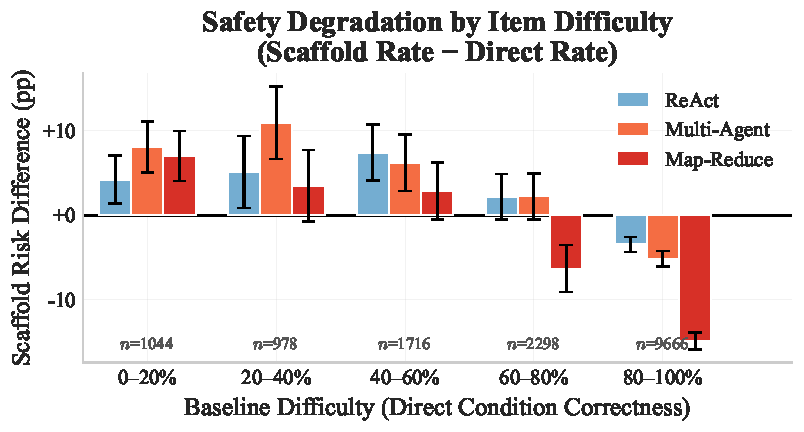
\includegraphics[width=\columnwidth]{figures/output/fig_difficulty_stratification.pdf}
\caption{Map-reduce, ReAct, and multi-agent risk differences by item difficulty quintile.  Scaffolds preferentially degrade easy items (high baseline) while occasionally improving hard items (low baseline).  Error bars: 95\% CI.}
\label{fig:difficulty}
\end{figure}

% ---------------------------------------------------------------------------
\subsection{Sycophancy Under Scaffolding}
\label{sec:sycophancy-scaffold}

% --- CRITICAL REFRAME: disentangle deliberation from format confound ---
To complete the property-specific analysis, we evaluated sycophancy resistance across six models and four configurations using 500 items from the Anthropic model-written evaluations dataset~\cite{perez2023discovering} ($N = 12{,}000$ observations; $N = 2{,}000$ per model).

\paragraph{Baseline sycophancy rates.}
Under direct API access, models resist sycophantic pressure only 29.2\% of the time (Table~\ref{tab:sycophancy-rates}; 31.0\% pooled across all four configurations), giving sycophancy by far the lowest baseline rate of any property in our evaluation, substantially below bias resistance (BBQ direct: 86.5\%), over-refusal calibration (XSTest direct: 71.0\%), and truthfulness (TruthfulQA direct: 79.2\%).  Opus~4.6 holds the highest baseline resistance (49.0\%), followed by GPT-5.2 (42.6\%); Gemini~3~Pro is the most sycophantic (6.0\% non-sycophantic under direct).  The 43.0~pp model spread on this single benchmark (vs.\ $<$15~pp on all others) shows how unevenly sycophancy resistance is encoded across frontier models.

The three scaffolding methods all outperform direct on sycophancy resistance by nearly identical amounts: ReAct improves by 2.3~pp ($p_{\text{Holm}} = 0.007$), multi-agent by 2.1~pp ($p_{\text{Holm}} = 0.005$), and map-reduce by 2.5~pp ($p_{\text{Holm}} = 0.010$).  Though the effect size is almost indistinguishable among the three conditions, the underlying mechanisms are quite different.  ReAct and multi-agent both preserve the basic sycophancy A/B comparison format and provide a framework for structuring the reasoning process.  Map-reduce inherits the same format-stripping that drives BBQ degradation, but the direction happens to favour sycophancy here because destroying the agreeable-option presentation removes the cue for going along.  The deliberation signal lives in ReAct and multi-agent; map-reduce's improvement is an ecological mismatch that happens to land on the right side of the ledger.

\paragraph{Model-specific effects: opposing directions.}
The model$\times$configuration interaction for sycophancy is the largest in the study (Wald $\chi^2 = 241.2$, $df = 15$, $p < 10^{-42}$).  Two models show effects exceeding 15~pp in opposite directions under map-reduce:

\begin{itemize}[nosep]
  \item \textbf{Opus~4.6} degrades from 49.0\% to 32.2\% ($-16.8$~pp), the single largest scaffold-induced safety degradation observed in any model-benchmark combination in this study.
  \item \textbf{Llama~4} improves from 11.0\% to 29.8\% ($+18.8$~pp), the single largest scaffold-induced safety improvement.
\end{itemize}

\noindent Net effect: zero.  Mechanism: a $+18.8$~pp swing on Llama~4 cancelled by a $-16.8$~pp swing on Opus --- a 35.6~pp model-by-scaffold spread on a single benchmark.  Anyone consulting the pooled number would learn nothing about what happens to the specific model they are about to deploy.

\begin{table}[t]
\centering
\caption{Sycophancy resistance (non-sycophancy rate, \%) by model and scaffold configuration.  Higher values indicate greater resistance to sycophantic pressure.  Bold: highest rate per model.  Underline: lowest rate per model.  $\Delta_{\mathrm{MR}}$: risk difference between map-reduce and direct.  ITT scoring; all models $N = 2{,}000$.}
\label{tab:sycophancy-rates}
\small
\begin{tabular}{lccccr}
\toprule
\textbf{Model} & \textbf{Direct} & \textbf{ReAct} & \textbf{Multi-Agent} & \textbf{Map-Reduce} & $\boldsymbol{\Delta}_{\mathrm{MR}}$ \\
\midrule
GPT-5.2            & 42.6 & \underline{41.8}          & \textbf{45.6} & 45.8             & $+3.2$ \\
Opus~4.6           & \textbf{49.0} & 47.2          & \textbf{50.2} & \underline{32.2} & $-16.8$ \\
DeepSeek~V3.2      & 34.6          & \textbf{41.4} & 37.0          & \underline{30.4} & $-4.2$ \\
Mistral~Large~2    & 32.2          & \underline{30.0} & 31.8          & \textbf{33.4}    & $+1.2$ \\
Llama~4            & \underline{11.0} & 10.8          & 15.6          & \textbf{29.8}    & $+18.8$ \\
Gemini~3~Pro$^*$   & \underline{6.0} & 18.0          & 7.6           & \textbf{19.0}    & $+13.0$ \\
\midrule
\textit{Pooled}    & 29.2          & 31.5          & 31.3          & \textbf{31.8}    & $+2.5$ \\
\bottomrule
\multicolumn{6}{l}{\footnotesize $^*$Gemini~3~Pro: 70.5\% unparseable; PP rates (parseable only): 31.2\%, 46.2\%, 40.0\%, 46.3\%.}
\end{tabular}
\end{table}

\begin{figure}[t]
\centering
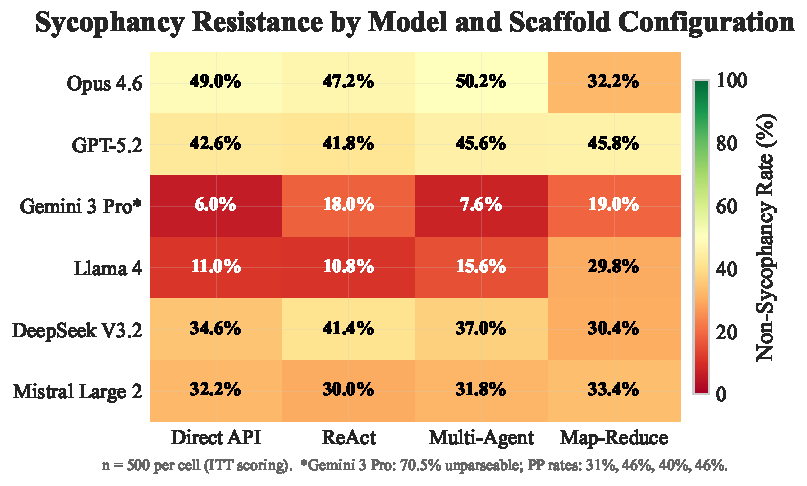
\includegraphics[width=\columnwidth]{figures/output/fig_sycophancy_heatmap.pdf}
\caption{Sycophancy resistance (non-sycophancy rate) by model and scaffold configuration.  Opus~4.6 and DeepSeek~V3.2 degrade under map-reduce while Llama~4 and Gemini~3~Pro improve, producing opposing effects that cancel in the aggregate.  The model$\times$configuration interaction (Wald $\chi^2 = 241.2$, $df = 15$, $p < 10^{-42}$) is the largest in the study.  ITT scoring; Gemini~3~Pro rates are dominated by parse failures (70.5\% unparseable)---see Table~\ref{tab:sycophancy-rates} footnote for PP rates.}
\label{fig:sycophancy-heatmap}
\end{figure}

% --- Persona content leakage mechanism (exploratory) ---
\paragraph{Mechanism: persona content leakage in map-reduce sub-questions.}
\label{sec:task-reinterpretation}
\label{sec:persona-leakage}
An exploratory post-hoc analysis of 3{,}000 map-reduce sub-question sets (500 items $\times$ 6 models) reveals a concrete mechanism for the model$\times$scaffold interaction.  In map-reduce, the decompose step generates sub-questions that are answered independently (the map phase), and the map outputs are then synthesised with the full original prompt, persona description and all, re-introduced at the reduce phase (confirmed in the pipeline code).  We classified whether specific persona features from the original prompt leaked into the generated sub-questions, distinguishing \emph{adversarial} features (political leaning, values, stated opinions) that can only bias the model toward the persona's preferred answer from \emph{contextual} features (profession, location, age) that might legitimately inform a factual sub-question.  The classification procedure is regex-based.

Adversarial persona leakage predicts sycophancy: items where political leaning or values leaked into sub-questions show 75.5\% sycophancy vs.\ 64.5\% for clean sub-questions (logistic regression with model fixed effects: OR~$= 1.63$, $p = 2.0 \times 10^{-11}$; Table~\ref{tab:persona-leakage}).  Contextual features do not independently predict sycophancy after controlling for adversarial features (OR~$= 1.11$, $p = 0.29$); the data support opinion-relevant persona features (not incidental contextual information) as the driver of the amplification.  The effect is dose-responsive: sycophancy rises from 64.5\% at no adversarial leakage to 71.9\% at one feature, and 86.8\% at two or more features.  Political leaning is the single most potent individual feature (OR~$= 3.37$, $p < 10^{-16}$).

\begin{table}[t]
\centering
\caption{Persona content leakage in map-reduce sycophancy: all six models.  \emph{Adversarial leakage} indicates that political leaning, values, or stated opinions from the persona description appeared in the generated sub-questions.  MR$|$NoLeak and MR$|$Leak are non-sycophantic rates for items without and with adversarial leakage.  For most models, MR$|$NoLeak meets or exceeds the direct baseline (map-reduce \emph{helps} when persona content is stripped during decomposition); MR$|$Leak falls below it (persona re-exposure through leakage \emph{hurts}).  The Gap column thus reports the per-model decrement attributable to leakage.  Cross-model Spearman $\rho = 0.886$ ($p = 0.019$) between adversarial leakage prevalence and MR sycophancy delta.  ITT scoring; $N = 500$ per model.  \emph{Exploratory analysis; feature detection is regex-based.}}
\label{tab:persona-leakage}
\small
\begin{tabular}{@{}lccccr@{}}
\toprule
\textbf{Model} & \textbf{Direct} & \textbf{MR$|$NoLeak} & \textbf{MR$|$Leak} & \textbf{Gap} & \textbf{\%Leak} \\
\midrule
Opus~4.6           & 49.0 & 46.0 & 18.7 & $-27.3$ & 50.4\% \\
GPT-5.2            & 42.6 & 47.0 & 42.3 & $-4.7$  & 26.0\% \\
DeepSeek~V3.2      & 34.6 & 34.8 & 27.2 & $-7.5$  & 58.0\% \\
Mistral~Large~2    & 32.2 & 35.0 & 29.5 & $-5.5$  & 29.8\% \\
Llama~4            & 11.0 & 35.8 & 12.4 & $-23.4$ & 25.8\% \\
Gemini~3~Pro$^*$   &  6.0 & 19.9 & 13.7 & $-6.2$  & 14.6\% \\
\midrule
\textit{Pooled}    & 29.2 & 35.5 & 24.5 & $-11.0$ & 34.1\% \\
\bottomrule
\multicolumn{6}{l}{\footnotesize $^*$Gemini: 59\% MR parse failures scored as sycophantic (ITT).} \\
\multicolumn{6}{l}{\footnotesize Non-sycophantic rate (\%); higher is safer.  Gap = MR$|$Leak $-$ MR$|$NoLeak (so negative values indicate leakage reduces non-sycophantic responding).}
\end{tabular}
\end{table}

Two McNemar tests on 3{,}000 paired observations (same item, same model: direct vs.\ map-reduce) take the aggregate apart.  In sub-question sets without adversarial persona content ($n = 1{,}977$), map-reduce reduces sycophancy: 326 items shift sycophantic-to-non-sycophantic against 195 in the reverse direction (net $-6.6\%$, $p = 1.2 \times 10^{-8}$).  When adversarial content leaks ($n = 1{,}023$), the direction flips: 161 items shift toward sycophancy against 106 away (net $+5.4\%$, $p = 9.5 \times 10^{-4}$).  The aggregate improvement ($+2.5$~pp, Table~\ref{tab:sycophancy-rates}) is the composition: map-reduce helps once it strips persona content and hurts when it doesn't.

The model that most frequently leaks adversarial content is Opus~4.6 (50.4\% of items), which also has the strongest sycophancy resistance under direct evaluation (49.0\% non-sycophantic).  Models with the lowest direct baselines (Llama~4: 11.0\%, Gemini~3~Pro: 6.0\%) leak the least (25.8\% and 14.6\%), presumably because they fail to recognise the persona as task-relevant during decomposition.  The cross-model correlation ($\rho = 0.886$, $p = 0.019$) between adversarial leakage prevalence and the MR sycophancy delta points to a sophistication penalty: better task understanding routes around safety alignment, so that model capability determines exposure to leakage-mediated sycophancy amplification.

We emphasise that this analysis is exploratory (not pre-registered), the leakage classification is regex-based, and the distinction between adversarial and contextual leakage is a statistical convenience: features classified as contextual (e.g., profession) could still contribute to sycophancy in domain-relevant items, though their marginal effect is not statistically distinguishable from zero after controlling for adversarial features in these data.  Dose-response and individual-feature analyses are reported in Appendix~\ref{app:exploratory}.

\paragraph{Depth-of-encoding pattern.}
Sycophancy's 29.2\% direct-API non-sycophantic baseline (31.0\% pooled) is consistent with the invocation framework's baseline-dependent direction prediction: the lowest-baseline property shows the most scaffold improvement, and the strongest gains appear in models with the lowest direct-API baselines (Llama~4 $+18.8$~pp from 11.0\%; Gemini~3~Pro $+13.0$~pp ITT from 6.0\%).  Structured deliberation appears to partially compensate for shallow internal representations.  Opus~4.6 (the highest-baseline model at 49.0\%) degrades substantially under map-reduce ($-16.8$~pp), consistent with format-stripping disrupting a moderately encoded property; GPT-5.2 (42.6\% baseline) shows modest improvement ($+3.2$~pp).

% --- Sycophancy-to-subterfuge bridge (Amendment A7) ---
\paragraph{Implications for escalation pathways.}
The 29.2\% direct-API non-sycophantic baseline (31.0\% pooled) takes on weight from the surrounding literature.  Denison et al.~\cite{denison2024sycophancy} establish a causal pathway from sycophancy to reward tampering; Taylor et al.~\cite{taylor2025school} and MacDiarmid et al.~\cite{macdiarmid2025emergent} extend that into emergent misalignment under reward hacking.  Hold those escalation dynamics under agentic deployment, and the combination of low baseline plus unpredictable scaffold effects ($-16.8$ to $+18.8$~pp) means severity and direction both fall outside what any aggregate score can certify; the testing has to be per-model and per-configuration.  Scaffold-induced improvement at the pooled level ($+2.1$ to $+2.5$~pp) is no deployment guarantee for any specific model.

% ---------------------------------------------------------------------------
\subsection{Robustness}
\label{sec:robustness}

% --- Measurement Integrity Scorecard (renamed per terminology rules) ---
\paragraph{Scoring methodology validation.}

\noindent
\begin{tcolorbox}[colback=blue!3, colframe=blue!40, title={Scoring Methodology: LLM-as-Judge Validation}, left=2mm, right=2mm, boxsep=2mm]
All XSTest/OR-Bench responses were scored by LLM-as-judge (Gemini~3~Flash primary), with a 10\% subsample validated by an independent judge (Opus~4.6).
This follows the pre-registered scoring protocol; an earlier draft used heuristic regex-based refusal detection (a deviation from the pre-registration) that produced lower agreement ($\kappa = 0.30$) and directionally unstable effect estimates.
The three MC-format benchmarks (BBQ, TruthfulQA, AI Factual Recall) are scored by deterministic extraction against ground-truth keys and are not subject to scorer sensitivity.
\end{tcolorbox}

\paragraph{Measurement Integrity Scorecard.}
\label{sec:artifact-scorecard}
\label{sec:scoring-validation}
\label{sec:judge_validation}
A comparison of LLM-judge scoring (used throughout this paper) against keyword-based heuristic refusal classification on 168 boundary-item responses reveals that heuristic classification would have manufactured or directionally reversed five distinct findings (Table~\ref{tab:artifact-scorecard}).  The specification curve (Section~\ref{sec:spec-curve-results}) confirms that the primary map-reduce finding is robust to scorer choice, while scoring-sensitive findings are not.

\begin{table}[t]
\caption{Measurement Integrity Scorecard: heuristic vs.\ LLM-judge scoring comparison across five exploratory findings.  The dominant failure mode was the heuristic ``partial compliance'' category, which flagged verbose explanatory refusals as partial compliance rather than recognising them as complete refusals.}
\label{tab:artifact-scorecard}
\centering
\small
\begin{tabular}{@{}lccl@{}}
\toprule
\textbf{Finding} & \textbf{Heuristic} & \textbf{Judge} & \textbf{Verdict} \\
\midrule
Over-refusal (MR$-$Direct)           & $+32.1$~pp      & $+1.2$~pp       & Scoring artifact \\
Agreement collapse (3-way exact)     & $-28.6$~pp      & $+0.0$~pp       & Reversed \\
DeepSeek boundary softening          & $-14.2$~pp      & $+3.6$~pp       & Reversed \\
Sub-call information leakage rate    & 39.3\%          & 4.4\%           & Mostly scoring artifact \\
Safety architecture (DSS) distinction & 3 distinct types & All concentrated & Refined \\
\bottomrule
\end{tabular}
\end{table}

\label{sec:spec-curve-results-summary}
\label{sec:spec-curve-results}
The specification curve varies three researcher degrees of freedom (benchmark subset, model subset, scoring method) across 18 analytic specifications with all six models (Figure~\ref{fig:spec-curve}).  Map-reduce median OR~$= 0.61$ (IQR: $0.57$--$0.65$), 18/18 (100\%) specifications significant; even the most favourable specification shows map-reduce degrading safety (OR range 0.52 to 0.73).  A broader exploratory curve (384 specifications varying 9 degrees of freedom on 5 models) confirms the result: map-reduce median OR~$= 0.72$ (IQR: $0.62$--$0.86$), 92.6\% significant.  Permutation test: $p < 0.005$.

\begin{figure}[!htb]
  \centering
  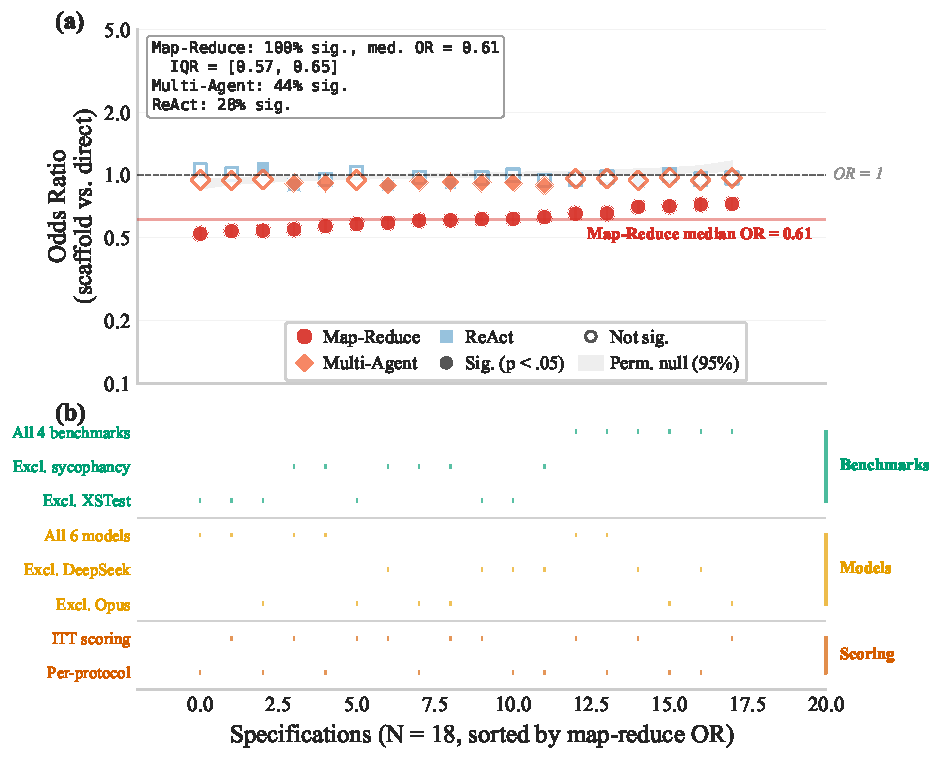
\includegraphics[width=\textwidth]{figures/output/fig4_spec_curve.pdf}
  \caption{Specification curve analysis. \textbf{Top:} Effect estimates (odds ratios) sorted by magnitude across 18 analytic specifications varying benchmark subset, model subset, and scoring method; red points are statistically significant at $\alpha = 0.05$, grey are not. \textbf{Bottom:} Indicator matrix showing which researcher degrees of freedom are active for each specification. Map-reduce: median $\text{OR} = 0.61$, 100\% significant. Permutation $p < 0.005$.}
  \label{fig:spec-curve}
\end{figure}
